
%(BEGIN_QUESTION)
% Copyright 2009, Tony R. Kuphaldt, released under the Creative Commons Attribution License (v 1.0)
% This means you may do almost anything with this work of mine, so long as you give me proper credit

Forklar hvordan følgende dypperør-system måler \textit{tetthet} av væsken i tanken i stedet for \textit{nivå}.  Anta at væskenivået aldri faller under øvre dypperør, og at høydeforskjellen mellom de to dypperørene er fast 12 tommer (1 fot):

$$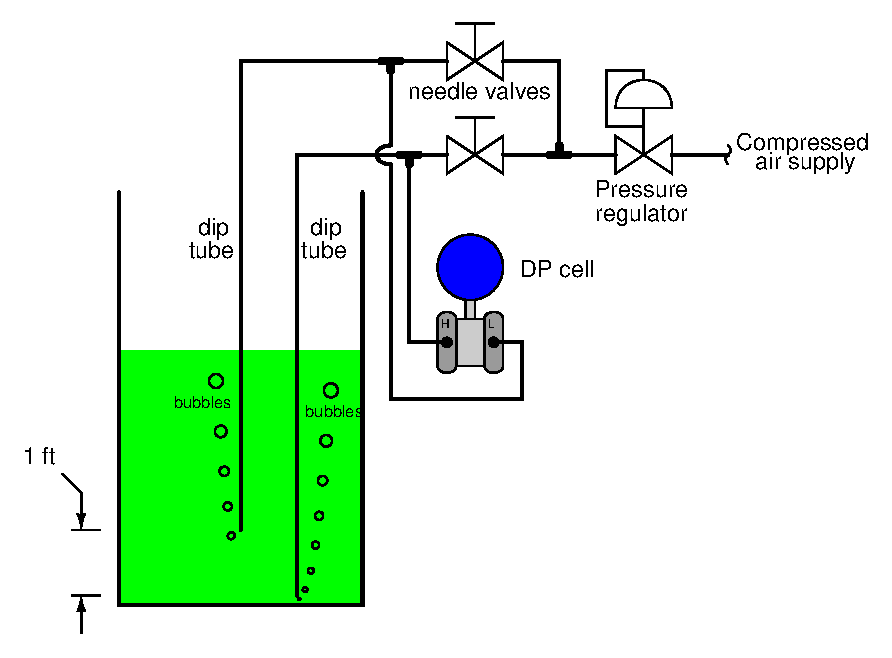
\includegraphics[width=15.5cm]{i00264x01.eps}$$

Beregn også differansetrykket DP-transmitteren måler for en væske med tetthet 58 pund per kubikkfot.

\vfil

\underbar{file i00264}
\eject
%(END_QUESTION)





%(BEGIN_ANSWER)

Dette er en gradert oppgave -- ingen svar eller hint oppgis!

%(END_ANSWER)





%(BEGIN_NOTES)

Så lenge begge dypperørene er neddykket, er den eneste variable som påvirker differansetrykket væsketetthet (fordi høydeforskjellen mellom rørene er konstant).

\vskip 10pt

Trykk = 11.15 inches water column (0.4028 PSID) ved væsketetthet 58 lb/ft$^{3}$.

%INDEX% Measurement, density: bubble tube (bubbler)
%INDEX% Measurement, density: dip tube (bubbler)
%INDEX% Measurement, density: hydrostatic pressure

%(END_NOTES)
